% 4.3-4.6 Study Guide -- September 2026
%
% Questions, then the answer key, then the source list -- ONE file (see WORKFLOW.md).
% Figures are cropped screenshots, not TikZ: fig-4.3-4.6-q14.png, fig-4.3-4.6-q16.png, fig-4.3-4.6-q17.png and
% fig-4.3-4.6-q18.png must sit in the same Overleaf project folder as this .tex.
%
% WORK SPACE: change the four lengths in \wsS \wsM \wsL \wsG below to make every
% blank on the worksheet bigger or smaller at once.
%
\documentclass[11pt]{article}
\usepackage[margin=1in]{geometry}
\usepackage{amsmath,amssymb}
\usepackage{enumitem}
\usepackage{graphicx}
\usepackage{multicol}

% ---- blank space for students to work in ----
\newcommand{\wsS}{\vspace*{3cm}}    % one- or two-step problem
\newcommand{\wsM}{\vspace*{4.5cm}}  % several steps, or parts (a)(b)(c)
\newcommand{\wsL}{\vspace*{6.5cm}}  % sketch a graph / long argument
\newcommand{\wsG}{\vspace*{2cm}}    % short answers beside a printed graph

\newlist{probs}{itemize}{1}
\setlist[probs]{leftmargin=2.6em,itemsep=6pt,topsep=4pt,label={}}
\newcommand{\prob}[1]{\item[\textbf{#1.}]}
\newcommand{\headnote}[1]{\smallskip\noindent\textit{#1}\par\nopagebreak}

\newlist{ans}{itemize}{1}
\setlist[ans]{leftmargin=3.2em,itemsep=4pt,topsep=4pt,label={}}
\newcommand{\ansitem}[1]{\item[\textbf{#1.}]}

% conditions list used by the "sketch a graph that satisfies..." problems
\newenvironment{conds}
  {\begin{list}{}{\leftmargin=1.2em\itemsep=1pt\topsep=3pt\parsep=0pt}\item[]}
  {\end{list}}

\title{\textbf{4.3--4.6 Study Guide}}
\author{}
\date{September 2026}

\begin{document}
\maketitle
\vspace{-2.5em}
\begin{center}\small Recommended Continued Practice (not for credit)\end{center}
\vspace{1em}

\headnote{Find the local extrema of $f$ and the intervals on which $f$ is increasing or is
decreasing, and sketch the graph of $f$.}
\begin{probs}
  \prob{1} $f(x)=10x^{3}(x-1)^{2}$ \wsL
\end{probs}

\headnote{Find the local extrema of $f$ on $[0,2\pi]$ and the subintervals on which $f$ is
increasing or is decreasing. Sketch the graph of $f$.}
\begin{probs}
  \prob{2} $f(x)=\tfrac{1}{2}x-\sin x$ \wsL
\end{probs}

\clearpage

\headnote{Find the local extrema of $f$, using the second derivative test whenever
applicable. Find the intervals on which the graph of $f$ is concave upward or is concave
downward, and find the $x$-coordinates of the points of inflection. Sketch the graph
of $f$.}
\begin{probs}
  \prob{3} $f(x)=\sqrt[5]{x}-1$ \wsL

  \prob{4} $f(x)=\sqrt[3]{x^{2}}\,(3x+10)$ \wsL
\end{probs}

\clearpage

\headnote{Sketch the graph of a continuous function $f$ that satisfies all of the stated
conditions.}
\begin{probs}
  \prob{5}
  \begin{conds}
    $f(0)=3$;\quad $f(-2)=f(2)=-4$;\quad $f'(0)$ is undefined;\\
    $f'(-2)=f'(2)=0$;\quad $f'(x)>0$ if $-2<x<0$ or $x>2$;\\
    $f'(x)<0$ if $x<-2$ or $0<x<2$
  \end{conds}
  \wsL

  \prob{6}
  \begin{conds}
    $f(0)=1$;\quad $f(2)=3$;\quad $f'(0)=f'(2)=0$;\\
    $f'(x)<0$ if $|x-1|>1$;\quad $f'(x)>0$ if $|x-1|<1$;\\
    $f''(x)>0$ if $x<1$;\quad $f''(x)<0$ if $x>1$
  \end{conds}
  \wsL
\end{probs}

\clearpage

\begin{probs}
  \prob{7}
  \begin{conds}
    $f(0)=2$;\quad $f(2)=f(-2)=1$;\quad $f'(0)=0$;\\
    $f'(x)>0$ if $x<0$;\quad $f'(x)<0$ if $x>0$;\\
    $f''(x)<0$ if $|x|<2$;\quad $f''(x)>0$ if $|x|>2$
  \end{conds}
  \wsL

  \prob{8}
  \begin{conds}
    $f(1)=4$;\quad $f'(x)>0$ if $x<1$;\quad $f'(x)<0$ if $x>1$;\\
    $f''(x)>0$ for every $x\neq 1$
  \end{conds}
  \wsL
\end{probs}

\clearpage

\begin{probs}
  \prob{9} If $n$ is an odd integer, then $f(n)=1$ and $f'(n)=0$; if $n$ is an even
  integer, then $f(n)=0$ and $f'(n)$ does not exist; if $n$ is any integer, then
  \begin{enumerate}[label=\textbf{(\alph*)},leftmargin=2.4em,itemsep=2pt,topsep=4pt]
    \item $f'(x)>0$ whenever $2n<x<2n+1$
    \item $f'(x)<0$ whenever $2n-1<x<2n$
    \item $f''(x)<0$ whenever $2n<x<2n+2$
  \end{enumerate}
  \wsL
\end{probs}

\headnote{Find the extrema and points of inflection, and sketch the graph of $f$.}
\begin{probs}
  \prob{10} $f(x)=\dfrac{3x}{(x+8)^{2}}$ \wsL
\end{probs}

\clearpage

\headnote{Simplify $f(x)$ and sketch the graph of $f$.}
\begin{probs}
  \prob{11} $f(x)=\dfrac{x-1}{1-x^{2}}$ \wsL
\end{probs}

\headnote{Sketch the graph of $f$.}
\begin{probs}
  \prob{12} $f(x)=\left|x^{3}+1\right|$ \wsL
\end{probs}

\clearpage

\begin{probs}
  \prob{13} A builder intends to construct a storage shed having a volume of
  $900\ \text{ft}^{3}$, a flat roof, and a rectangular base whose width is three-fourths
  the length. The cost per square foot of the materials is \$4 for the floor, \$6 for the
  sides, and \$3 for the roof. What dimensions will minimize the cost?
  \wsL

  \prob{14} A steel storage tank for propane gas is to be constructed in the shape of a
  right circular cylinder with a hemisphere at each end (see figure). The construction
  cost per square foot for the end pieces is twice that for the cylindrical piece. If the
  desired capacity is $10\pi\ \text{ft}^{3}$, what dimensions will minimize the cost of
  construction?

  \smallskip
  \noindent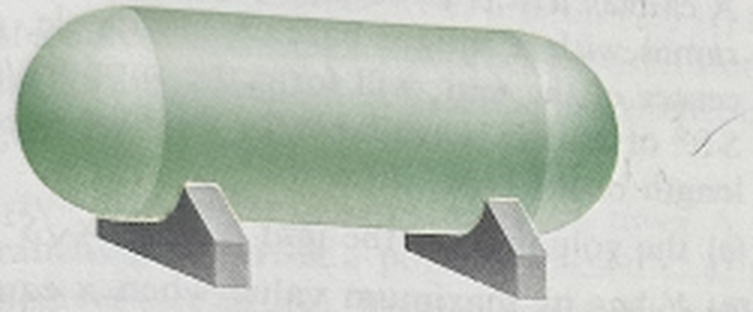
\includegraphics[width=0.45\linewidth]{fig-4.3-4.6-q14.png}
  \wsM
\end{probs}

\clearpage

\begin{probs}
  \prob{15} Find the point on the graph of $y=x^{2}+1$ that is closest to the point
  $(3,1)$.
  \wsL

  \prob{16} The strength of a rectangular beam is directly proportional to the product of
  its width and the square of the depth of a cross section. Find the dimensions of the
  strongest beam that can be cut from a cylindrical log of radius $a$ (see figure).

  \smallskip
  \noindent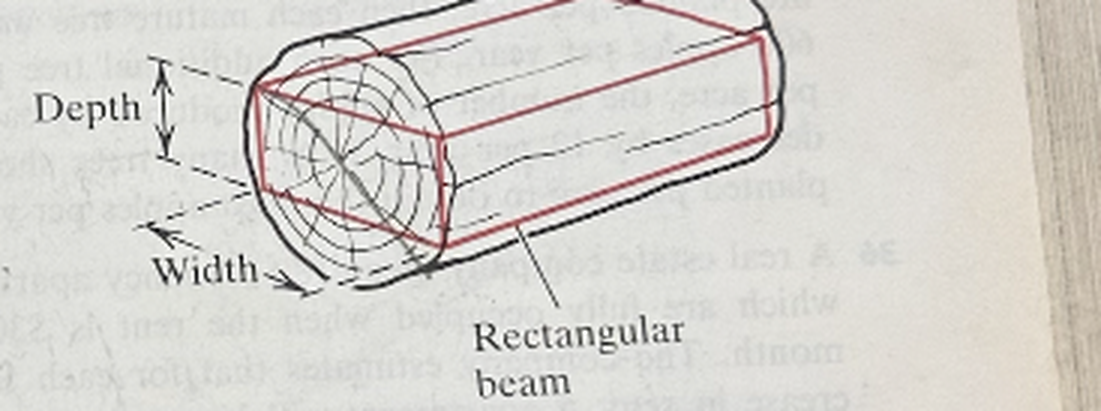
\includegraphics[width=0.55\linewidth]{fig-4.3-4.6-q16.png}
  \wsM
\end{probs}

\clearpage

\begin{probs}
  \prob{17} A battery having fixed voltage $V$ and fixed internal resistance $r$ is
  connected to a circuit that has variable resistance $R$ (see figure). By Ohm's law, the
  current $I$ in the circuit is $I=V/(R+r)$. If the power output $P$ is given by
  $P=I^{2}R$, show that the maximum power occurs if $R=r$.

  \smallskip
  \noindent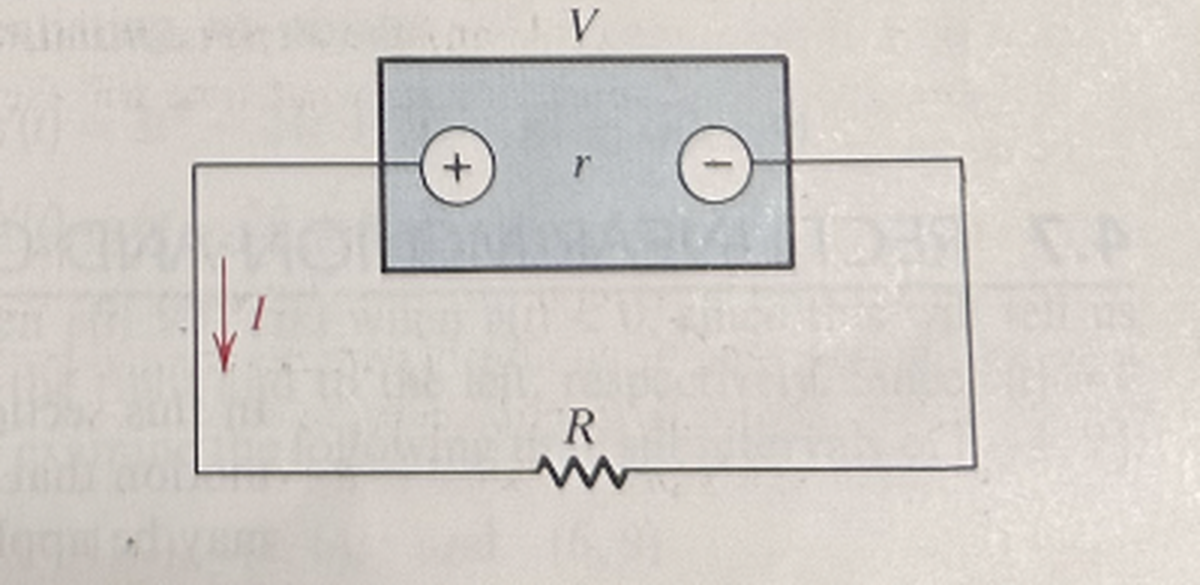
\includegraphics[width=0.52\linewidth]{fig-4.3-4.6-q17.png}
  \wsM
\end{probs}

\begin{probs}
  \prob{18} Two corridors 3 feet and 4 feet wide, respectively, meet at a right angle.
  Find the length of the longest nonbendable rod that can be carried horizontally around
  the corner, as shown in the figure. (Disregard the thickness of the rod.)

  \smallskip
  \noindent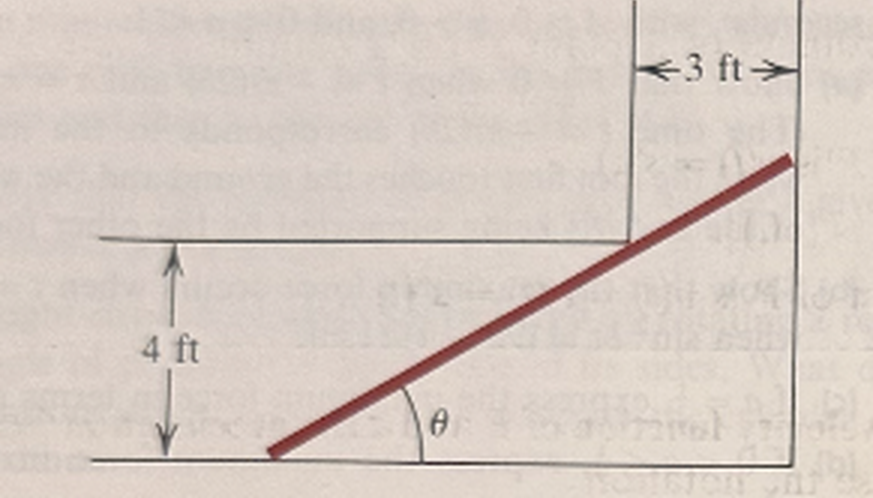
\includegraphics[width=0.45\linewidth]{fig-4.3-4.6-q18.png}
  \wsM
\end{probs}

\clearpage
%======================================================================
\section*{Tommy's Questions}
\noindent\textit{These three are written by us. Each one pulls several ideas together at
once, so show all of your work.}
\medskip

\noindent\textbf{Tommy 1.}\quad Let $f(x)=3x^{5}-20x^{3}+60x$.
\begin{enumerate}[label=\textbf{(\alph*)},leftmargin=2.8em,itemsep=6pt,topsep=5pt]
  \item Find $f'(x)$ and every critical number of $f$. \wsM
  \item Find the intervals on which $f$ is increasing and those on which $f$ is
        decreasing, and find every local extremum of $f$. \wsM
  \item Apply the second derivative test at each critical number found in part (a), and
        state what it tells you about that number. \wsM
  \item Find the intervals on which the graph of $f$ is concave upward and those on which
        it is concave downward, find the $x$-coordinates of all points of inflection, and
        sketch the graph of $f$. \wsL
\end{enumerate}

\clearpage

\noindent\textbf{Tommy 2.}\quad Find the minimum value of
\[
  f(x)=\bigl(x^{2}-6x+10\bigr)\bigl(x^{2}-6x+13\bigr)\bigl(x^{2}-6x+18\bigr).
\]
\wsL
\wsL

\clearpage

\noindent\textbf{Tommy 3.}\quad Find the minimum value of
\[
  f(x)=\frac{x^{4}+2x^{3}+5x^{2}+4x+8}{x^{2}+x+2}\,.
\]
\wsL
\wsL

\clearpage
%======================================================================
\begin{center}\Large\textbf{Answer Key}\end{center}
\medskip
\noindent\textit{Answers only for 1--18. Tommy's questions are worked in full.}
\medskip

\begin{ans}
  \ansitem{1} Increasing on $\left(-\infty,\tfrac{3}{5}\right]$ and $[1,\infty)$;
    decreasing on $\left[\tfrac{3}{5},1\right]$. Local maximum
    $f\!\left(\tfrac{3}{5}\right)=\tfrac{216}{625}=0.3456$; local minimum $f(1)=0$.
    ($x=0$ is a critical number but not an extremum: $f'$ does not change sign there.)

  \ansitem{2} Decreasing on $\left[0,\tfrac{\pi}{3}\right]$ and
    $\left[\tfrac{5\pi}{3},2\pi\right]$; increasing on
    $\left[\tfrac{\pi}{3},\tfrac{5\pi}{3}\right]$. Local minimum
    $f\!\left(\tfrac{\pi}{3}\right)=\tfrac{\pi}{6}-\tfrac{\sqrt3}{2}\approx-0.342$;
    local maximum
    $f\!\left(\tfrac{5\pi}{3}\right)=\tfrac{5\pi}{6}+\tfrac{\sqrt3}{2}\approx3.484$.

  \ansitem{3} No local extrema; $f$ is increasing on $(-\infty,\infty)$. Concave upward on
    $(-\infty,0)$, concave downward on $(0,\infty)$. Point of inflection $(0,-1)$, where
    the graph has a vertical tangent line.

  \ansitem{4} Local maximum $f\!\left(-\tfrac{4}{3}\right)=4\sqrt[3]{6}\approx7.27$;
    local minimum $f(0)=0$ (the second derivative test does not apply at $x=0$, since
    $f''(0)$ does not exist --- use the first derivative test). Concave downward on
    $(-\infty,0)$ and $\left(0,\tfrac{2}{3}\right)$; concave upward on
    $\left(\tfrac{2}{3},\infty\right)$. Point of inflection
    $\left(\tfrac{2}{3},\,4\sqrt[3]{12}\right)\approx(0.67,\,9.16)$. The graph has a cusp
    at the origin.

  \ansitem{5} Decreasing on $(-\infty,-2)$, increasing on $(-2,0)$, decreasing on $(0,2)$,
    increasing on $(2,\infty)$. Local minima $(-2,-4)$ and $(2,-4)$; local maximum
    $(0,3)$. Because $f'(0)$ does not exist, the graph must come to a sharp point at
    $(0,3)$ --- a corner or a cusp, not a smooth peak.

  \ansitem{6} Decreasing on $(-\infty,0)$, increasing on $(0,2)$, decreasing on
    $(2,\infty)$. Local minimum $(0,1)$; local maximum $(2,3)$. Concave upward on
    $(-\infty,1)$, concave downward on $(1,\infty)$; point of inflection at $x=1$ (its
    height is not determined by the conditions --- any value between $1$ and $3$ works).

  \ansitem{7} Increasing on $(-\infty,0)$, decreasing on $(0,\infty)$; local maximum
    $(0,2)$. Concave upward on $(-\infty,-2)$ and $(2,\infty)$, concave downward on
    $(-2,2)$. Points of inflection $(-2,1)$ and $(2,1)$.

  \ansitem{8} Increasing on $(-\infty,1)$, decreasing on $(1,\infty)$; local maximum
    $(1,4)$. The graph is concave upward on $(-\infty,1)$ and on $(1,\infty)$. Because it
    is concave upward on \emph{both} sides of the high point, $f$ cannot be differentiable
    at $x=1$: the graph must come to a corner (or cusp) at $(1,4)$, not a smooth hump.

  \ansitem{9} A repeating pattern of period $2$. Each arch starts at $(2n,0)$, rises to a
    smooth high point $(2n+1,1)$ with a horizontal tangent, and falls back to $(2n+2,0)$;
    it is concave downward the whole way. At every even integer two arches meet in a
    corner, so $f'$ does not exist there. The graph looks like
    $y=\left|\sin\frac{\pi x}{2}\right|$.

  \ansitem{10} Local maximum $\left(8,\tfrac{3}{32}\right)$; no local minimum. Concave
    downward on $(-\infty,-8)$ and $(-8,16)$; concave upward on $(16,\infty)$. Point of
    inflection $\left(16,\tfrac{1}{12}\right)$. Vertical asymptote $x=-8$; horizontal
    asymptote $y=0$.

  \ansitem{11} $f(x)=\dfrac{-1}{x+1}$ for $x\neq1$ and $x\neq-1$. So the graph is the
    graph of $y=-\dfrac{1}{x+1}$ with a \emph{hole} at $\left(1,-\tfrac{1}{2}\right)$.
    Vertical asymptote $x=-1$; horizontal asymptote $y=0$.

  \ansitem{12} The graph of $y=x^{3}+1$ with the piece below the $x$-axis (that is,
    $x<-1$) reflected up across the $x$-axis. Decreasing on $(-\infty,-1)$, increasing on
    $(-1,\infty)$; absolute minimum $(-1,0)$, which is a corner. Concave upward on
    $(-\infty,-1)$, concave downward on $(-1,0)$, concave upward on $(0,\infty)$. Point of
    inflection $(0,1)$. ($x=-1$ is \emph{not} a point of inflection: the concavity changes
    there, but there is no tangent line.)

  \ansitem{13} Length $=2\sqrt[3]{300}\approx13.39$ ft, width
    $=\tfrac{3}{2}\sqrt[3]{300}\approx10.04$ ft, height $=\sqrt[3]{300}\approx6.69$ ft.
    (Minimum cost $=630\sqrt[3]{90}\approx\$2823.29$.)

  \ansitem{14} Radius $r=\tfrac{1}{2}\sqrt[3]{15}\approx1.23$ ft; length of the
    cylindrical piece $L=2\sqrt[3]{15}\approx4.93$ ft. (Note $L=4r$; the tank is
    $3\sqrt[3]{15}\approx7.40$ ft long overall.)

  \ansitem{15} The point $(1,2)$; the distance is $\sqrt5\approx2.236$.

  \ansitem{16} Width $=\dfrac{2\sqrt3}{3}\,a\approx1.155a$ and depth
    $=\dfrac{2\sqrt6}{3}\,a\approx1.633a$; that is, depth $=\sqrt2\,\times$ width.

  \ansitem{17} $P=\dfrac{V^{2}R}{(R+r)^{2}}$, so
    $\dfrac{dP}{dR}=\dfrac{V^{2}(r-R)}{(R+r)^{3}}$, which is positive for $R<r$ and
    negative for $R>r$. Hence $P$ is largest at $R=r$, and the maximum power is
    $\dfrac{V^{2}}{4r}$.

  \ansitem{18} $\left(3^{2/3}+4^{2/3}\right)^{3/2}\approx9.87$ ft.
\end{ans}

\bigskip
\noindent\textbf{Tommy 1.}\quad $f(x)=3x^{5}-20x^{3}+60x$.
\begin{enumerate}[label=\textbf{(\alph*)},leftmargin=2.8em,itemsep=8pt,topsep=5pt]
  \item
  \[
    f'(x)=15x^{4}-60x^{2}+60=15\bigl(x^{4}-4x^{2}+4\bigr)=15\bigl(x^{2}-2\bigr)^{2}.
  \]
  $f'$ is defined for every $x$, so the critical numbers are the zeros of $f'$:
  $x=\sqrt2$ and $x=-\sqrt2$.

  \item $\bigl(x^{2}-2\bigr)^{2}$ is a square, so $f'(x)\ge0$ for \emph{every} $x$, with
  equality only at $x=\pm\sqrt2$. The derivative therefore never changes sign:
  \[
    f\ \text{is increasing on}\ (-\infty,\infty),\qquad\text{and $f$ has \textbf{no} local
    extrema.}
  \]
  Both critical numbers fail the first derivative test. A horizontal tangent line is not
  the same thing as a high or low point --- at $\left(\pm\sqrt2,\pm32\sqrt2\right)$ the
  graph flattens out for an instant and then keeps climbing.

  \item
  \[
    f''(x)=60x^{3}-120x=60x\bigl(x^{2}-2\bigr),
  \]
  so $f''\!\left(\sqrt2\right)=60\sqrt2\,(2-2)=0$ and likewise
  $f''\!\left(-\sqrt2\right)=0$. The second derivative test is \textbf{inconclusive at
  both critical numbers} --- it gives no information at all. This is exactly the situation
  the test is not built for, and part (b) is what settles the question.

  \item Factor: $f''(x)=60x\bigl(x-\sqrt2\bigr)\bigl(x+\sqrt2\bigr)$. Sign chart:
  \[
    \begin{array}{c|cccc}
      \text{interval} & \left(-\infty,-\sqrt2\right) & \left(-\sqrt2,0\right)
        & \left(0,\sqrt2\right) & \left(\sqrt2,\infty\right)\\\hline
      f'' & - & + & - & +\\
      \text{graph} & \text{concave down} & \text{concave up} & \text{concave down}
        & \text{concave up}
    \end{array}
  \]
  The concavity changes at all three zeros, so the points of inflection are
  \[
    \left(-\sqrt2,\,-32\sqrt2\right),\qquad(0,0),\qquad\left(\sqrt2,\,32\sqrt2\right),
  \]
  since $f\!\left(\sqrt2\right)=12\sqrt2-40\sqrt2+60\sqrt2=32\sqrt2\approx45.25$ and $f$ is
  an odd function.

  \medskip
  \textbf{Sketch.} An odd, everywhere-increasing curve through the origin, running from
  $-\infty$ to $+\infty$, with horizontal tangents at $\left(-\sqrt2,-32\sqrt2\right)$ and
  $\left(\sqrt2,32\sqrt2\right)$. Those two horizontal tangents are points of
  \emph{inflection}, not extrema --- which is the whole point of the problem.
\end{enumerate}

\bigskip
\noindent\textbf{Tommy 2.}\quad Answer: the minimum value is $\boxed{36}$, attained at
$x=3$.

\medskip
\noindent\textbf{The way in.} Every one of the three factors starts with the same
$x^{2}-6x$. Complete the square once and it appears in all three:
\[
  x^{2}-6x+10=(x-3)^{2}+1,\qquad
  x^{2}-6x+13=(x-3)^{2}+4,\qquad
  x^{2}-6x+18=(x-3)^{2}+9 .
\]
So if we write $t=(x-3)^{2}$, then
\[
  f(x)=(t+1)(t+4)(t+9),\qquad\text{where } t\ge0 .
\]

\medskip
\noindent\textbf{Finish.} Each of $t+1$, $t+4$, $t+9$ is positive and increasing for
$t\ge0$, so their product is increasing for $t\ge0$. The product is therefore smallest at
the smallest allowed $t$, namely $t=0$, and $t=(x-3)^{2}=0$ exactly when $x=3$:
\[
  f(3)=(0+1)(0+4)(0+9)=36 .
\]
No differentiation was needed at all.

\medskip
\noindent\textbf{What brute force costs.} Expanding gives
\[
  f(x)=x^{6}-18x^{5}+149x^{4}-708x^{3}+2020x^{2}-3264x+2340,
\]
and then
\[
  f'(x)=2(x-3)\bigl(x^{2}-6x+16\bigr)\bigl(3x^{2}-18x+34\bigr).
\]
The two quadratics have discriminants $-28$ and $-84$, so neither has a real zero and
$x=3$ really is the only real critical number. Same answer --- after a page of expansion
and a quintic to factor.

\medskip
\noindent\textbf{The trap.} Treating the three factors as if they compete with one
another, and hunting for a compromise value of $x$. They do not compete: all three bottom
out at the same place, $x=3$, because all three are built on the same $(x-3)^{2}$.

\bigskip
\noindent\textbf{Tommy 3.}\quad Answer: the minimum value is $\boxed{4}$, attained at
$x=0$ and at $x=-1$.

\medskip
\noindent\textbf{The way in.} Square the denominator and compare it with the numerator:
\[
  \bigl(x^{2}+x+2\bigr)^{2}=x^{4}+2x^{3}+5x^{2}+4x+4,
\]
which is the numerator less $4$. So writing $u=x^{2}+x+2$,
\[
  f(x)=\frac{u^{2}+4}{u}=u+\frac{4}{u}\,.
\]
One substitution turns a quartic-over-quadratic into two terms.

\medskip
\noindent\textbf{What values can $u$ take?} Completing the square,
$u=\left(x+\tfrac{1}{2}\right)^{2}+\tfrac{7}{4}$, so $u\ge\tfrac{7}{4}$, and every value
$u\ge\tfrac{7}{4}$ is actually attained (as $x$ runs over the reals, $u$ runs continuously
from $\tfrac{7}{4}$ up to $\infty$).

\medskip
\noindent\textbf{Minimize $g(u)=u+\dfrac{4}{u}$ on $\left[\tfrac{7}{4},\infty\right)$.}
\[
  g'(u)=1-\frac{4}{u^{2}}=\frac{u^{2}-4}{u^{2}},
\]
which is negative for $\tfrac{7}{4}\le u<2$ and positive for $u>2$. So $g$ decreases and
then increases, with its minimum at $u=2$:
\[
  g(2)=2+\frac{4}{2}=4 .
\]
Since $2\ge\tfrac{7}{4}$, the value $u=2$ is available. Solving
$x^{2}+x+2=2$ gives $x(x+1)=0$, so $x=0$ or $x=-1$, and indeed
\[
  f(0)=\frac{8}{2}=4,\qquad f(-1)=\frac{1-2+5-4+8}{1-1+2}=\frac{8}{2}=4 .
\]

\medskip
\noindent\textbf{The two traps.}
\begin{enumerate}[label=\textbf{(\arabic*)},leftmargin=2.6em,itemsep=4pt,topsep=4pt]
  \item \emph{Minimizing $u$ instead of $f$.} The smallest $u$ occurs at
  $x=-\tfrac{1}{2}$, and there
  $f\!\left(-\tfrac{1}{2}\right)=\tfrac{7}{4}+\tfrac{16}{7}=\tfrac{113}{28}\approx4.036$,
  which is \emph{larger} than $4$. In fact $x=-\tfrac{1}{2}$ is a local \emph{maximum} of
  $f$, sitting between the two minima at $x=-1$ and $x=0$. Making the inside small does
  not make $u+\dfrac{4}{u}$ small.
  \item \emph{Forgetting to check that $u=2$ is reachable.} The unconstrained minimum of
  $u+\dfrac{4}{u}$ is at $u=2$, but that is only the answer because $2$ lies in the range
  $\left[\tfrac{7}{4},\infty\right)$. Had the range been $u\ge3$, the minimum would have
  been at the endpoint instead.
\end{enumerate}

\medskip
\noindent\textbf{What brute force costs.} The quotient rule, after simplifying, gives
\[
  f'(x)=\frac{x(x+1)(2x+1)\bigl(x^{2}+x+4\bigr)}{\bigl(x^{2}+x+2\bigr)^{2}},
\]
whose real zeros are $x=-1$, $x=-\tfrac{1}{2}$ and $x=0$ --- the same three points, after
a great deal more algebra.

\clearpage
% === SOURCELIST ===
%======================================================================
\begin{center}\Large\textbf{Where These Questions Came From}\end{center}
\medskip

\noindent These questions come from Sections 4.3, 4.4, 4.5 and 4.6 of the textbook. If you
got one wrong, look it up and try the problems around it --- that is where the extra
practice is.
\medskip

\begin{multicols}{2}
\noindent\textbf{Section 4.3}
\begin{itemize}[leftmargin=1.6em,itemsep=1pt,topsep=2pt]
  \item[] \textbf{1} $=$ 4.3 \#7
  \item[] \textbf{2} $=$ 4.3 \#19
  \item[] \textbf{5} $=$ 4.3 \#35
\end{itemize}

\smallskip
\noindent\textbf{Section 4.4}
\begin{itemize}[leftmargin=1.6em,itemsep=1pt,topsep=2pt]
  \item[] \textbf{3} $=$ 4.4 \#9
  \item[] \textbf{4} $=$ 4.4 \#11
  \item[] \textbf{6} $=$ 4.4 \#31
  \item[] \textbf{7} $=$ 4.4 \#33
  \item[] \textbf{8} $=$ 4.4 \#34
  \item[] \textbf{9} $=$ 4.4 \#37
\end{itemize}

\smallskip
\noindent\textbf{Section 4.5}
\begin{itemize}[leftmargin=1.6em,itemsep=1pt,topsep=2pt]
  \item[] \textbf{10} $=$ 4.5 \#19
  \item[] \textbf{11} $=$ 4.5 \#27
  \item[] \textbf{12} $=$ 4.5 \#31
\end{itemize}

\smallskip
\noindent\textbf{Section 4.6}
\begin{itemize}[leftmargin=1.6em,itemsep=1pt,topsep=2pt]
  \item[] \textbf{13} $=$ 4.6 \#11
  \item[] \textbf{14} $=$ 4.6 \#17
  \item[] \textbf{15} $=$ 4.6 \#23
  \item[] \textbf{16} $=$ 4.6 \#25
  \item[] \textbf{17} $=$ 4.6 \#51
  \item[] \textbf{18} $=$ 4.6 \#53
\end{itemize}

\smallskip
\noindent\textbf{Tommy's Questions}
\begin{itemize}[leftmargin=1.6em,itemsep=1pt,topsep=2pt]
  \item[] \textbf{Tommy 1} --- original, not in the textbook
  \item[] \textbf{Tommy 2} --- original, not in the textbook
  \item[] \textbf{Tommy 3} --- original, not in the textbook
\end{itemize}
\end{multicols}

\end{document}
